\documentclass[%preprint,
notitlepage,
%superscriptaddress,
%groupedaddress,
%unsortedaddress,
%runinaddress,
%frontmatterverbose, 
%preprint,
%preprintnumbers,
%nofootinbib,
%nobibnotes,
%bibnotes,
 amsmath,amssymb,
 aps,
%pra,
%prb,
rmp,
%prstab,
%prstper,
%floatfix,
]{revtex4-2}  % defines the basic parameters of the document

% if you want a single-column, remove reprint

% allows special characters (including æøå)
\usepackage[utf8]{inputenc}
\usepackage[norsk]{babel}

%% note that you may need to download some of these packages manually, it depends on your setup.
%% I recommend downloading TeXMaker, because it includes a large library of the most common packages.

\usepackage{physics,amssymb}  % mathematical symbols (physics imports amsmath)
\usepackage{graphicx}         % include graphics such as plots
\usepackage{xcolor}           % set colors
\usepackage{hyperref}         % automagic cross-referencing (this is GODLIKE)
\usepackage{tikz}             % draw figures manually
\usetikzlibrary{tikzmark}
\usepackage{listings}         % display code
\usepackage{subfigure}        % imports a lot of cool and useful figure commands
\usepackage{cprotect}
\usepackage{float}
\usepackage{caption}

\setlength{\parindent}{0px}

%Ta med disse kommandoene
\newcommand{\nnode}[2]{\node (#1) at (#2) {#1};}    %Her defineres nnode kommandoen
\newcommand{\relnode}[2]{\draw (#2) node[fill,circle,scale=0.6]{} (#2);\node (#1) at (#2) {};}  %Her defineres relnode kommandoen

% defines the color of hyperref objects
% Blending two colors:  blue!80!black  =  80% blue and 20% black
\hypersetup{ % this is just my personal choice, feel free to change things
    colorlinks,
    linkcolor={red!50!black},
    citecolor={blue!50!black},
    urlcolor={blue!80!black}}
%
%% Defines the style of the programming listing
%% This is actually my personal template, go ahead and change stuff if you want
\lstnewenvironment{python}{
	\lstset{ %
		inputpath=,
		backgroundcolor=\color{white!95!black},
		basicstyle={\ttfamily\scriptsize},
		commentstyle=\color{orange},
		language=Python,
		numbers=left,
		stepnumber=1,
		morekeywords={True,False},
		tabsize=4,
		stringstyle=\color{green!55!black},
		frame=single,
		keywordstyle=\color{blue},
		showstringspaces=false,
		columns=fullflexible,
		keepspaces=true}
}{}

\lstnewenvironment{cpp}{
	\lstset{ %
		inputpath=,
		backgroundcolor=\color{white!95!black},
		basicstyle={\ttfamily\scriptsize},
		commentstyle=\color{orange},
		language=C++,
		numbers=left,
		stepnumber=1,
		morekeywords={True,False},
		tabsize=4,
		stringstyle=\color{green!55!black},
		frame=single,
		keywordstyle=\color{blue},
		showstringspaces=false,
		columns=fullflexible,
		keepspaces=true}
}{}

\lstnewenvironment{sql}{
	\lstset{ %
		inputpath=,
		backgroundcolor=\color{white!95!black},
		basicstyle={\ttfamily\scriptsize},
		commentstyle=\color{orange},
		language=SQL,
		numbers=left,
		stepnumber=1,
		morekeywords={True,False},
		tabsize=4,
		stringstyle=\color{green!55!black},
		frame=single,
		keywordstyle=\color{blue},
		showstringspaces=false,
		columns=fullflexible,
		keepspaces=true}
}{}

\lstset{literate=
  {á}{{\'a}}1 {é}{{\'e}}1 {í}{{\'i}}1 {ó}{{\'o}}1 {ú}{{\'u}}1
  {Á}{{\'A}}1 {É}{{\'E}}1 {Í}{{\'I}}1 {Ó}{{\'O}}1 {Ú}{{\'U}}1
  {à}{{\`a}}1 {è}{{\`e}}1 {ì}{{\`i}}1 {ò}{{\`o}}1 {ù}{{\`u}}1
  {À}{{\`A}}1 {È}{{\'E}}1 {Ì}{{\`I}}1 {Ò}{{\`O}}1 {Ù}{{\`U}}1
  {ä}{{\"a}}1 {ë}{{\"e}}1 {ï}{{\"i}}1 {ö}{{\"o}}1 {ü}{{\"u}}1
  {Ä}{{\"A}}1 {Ë}{{\"E}}1 {Ï}{{\"I}}1 {Ö}{{\"O}}1 {Ü}{{\"U}}1
  {â}{{\^a}}1 {ê}{{\^e}}1 {î}{{\^i}}1 {ô}{{\^o}}1 {û}{{\^u}}1
  {Â}{{\^A}}1 {Ê}{{\^E}}1 {Î}{{\^I}}1 {Ô}{{\^O}}1 {Û}{{\^U}}1
  {œ}{{\oe}}1 {Œ}{{\OE}}1 {æ}{{\ae}}1 {Æ}{{\AE}}1 {ß}{{\ss}}1
  {ű}{{\H{u}}}1 {Ű}{{\H{U}}}1 {ő}{{\H{o}}}1 {Ő}{{\H{O}}}1
  {ç}{{\c c}}1 {Ç}{{\c C}}1 {ø}{{\o}}1 {å}{{\r a}}1 {Å}{{\r A}}1
  {€}{{\euro}}1 {£}{{\pounds}}1 {«}{{\guillemotleft}}1
  {»}{{\guillemotright}}1 {ñ}{{\~n}}1 {Ñ}{{\~N}}1 {¿}{{?`}}1
}

\newcommand{\set}[1]{\ensuremath{\left\{#1\right\}}}
\newcommand{\tuple}[1]{\ensuremath{\left\langle #1 \right\rangle}}
\newcommand{\imp}{\ensuremath{\rightarrow}}

\newcommand{\ceil}[1]{\ensuremath{\lceil #1 \rceil}}
\newcommand{\floor}[1]{\ensuremath{\lfloor #1 \rfloor}}

\usepackage{thmtools}
\DeclareMathOperator{\nullspace}{Nul}
\DeclareMathOperator{\collspace}{Col}
\DeclareMathOperator{\rref}{Rref}
%%\DeclareMathOperator{\dim}{Dim}

 % "meq": must be equal
\newcommand{\meq}{\overset{!}{=}}
\newcommand\numberthis{\addtocounter{equation}{1}\tag{\theequation}}

\newcommand{\R}{\mathbb{R}}
\newcommand{\N}{\mathbb{N}}
\newcommand{\Z}{\mathbb{Z}}
\newcommand{\Q}{\mathbb{Q}}
\newcommand{\C}{\mathbb{C}}
\newcommand*\Heq{\ensuremath{\overset{\kern2pt L'H}{=}}}
\usepackage{bm}
\newcommand{\uveci}{{\bm{\hat{\textnormal{\bfseries\i}}}}}
\newcommand{\uvecj}{{\bm{\hat{\textnormal{\bfseries\j}}}}}
\DeclareRobustCommand{\uvec}[1]{{%
  \ifcsname uvec#1\endcsname
     \csname uvec#1\endcsname
   \else
    \bm{\hat{\mathbf{#1}}}%
   \fi
}}
\usepackage[binary-units=true]{siunitx}

\newcommand{\twopartdef}[4]
{
	\left\{
		\begin{array}{ll}
			#1 & \mbox{if } #2 \\
			#3 & \mbox{if } #4
		\end{array}
	\right.
}

\makeatletter
\newcommand*{\balancecolsandclearpage}{%
  \close@column@grid
  \cleardoublepage
  \twocolumngrid
}
\makeatother

\AtBeginEnvironment{align}{\setcounter{equation}{0}}
\newcounter{subproject}
\renewcommand{\thesubproject}{\alph{subproject}}
\newenvironment{subproj}{
\begin{description}
	\item[\refstepcounter{subproject}(\thesubproject)]
}{\end{description}}


\begin{document}
\title{Oblig 1}   % self-explanatory
\author{Anders P. Åsbø}               % self-explanatory
\date{\today}                             % self-explanatory
\noaffiliation                            % ignore this

\maketitle                                % creates the title, author, date

Til denne obligen brukte jeg en database som kjørte på Wampserver med MySQL 8.0.27, men jeg brukte JetBrains DataGrip til å faktisk skrive, samt kjøre SQL-koden og interagere med databasen.

\section*{Oppgave 1}
\subsection*{a)}
For å lage databasen "Oblig1" bruker jeg sql setningen
\begin{sql}
oblig1> CREATE SCHEMA Oblig1
[2022-09-11 16:51:14] 1 row affected in 9 ms
\end{sql}
Som resulterer i
\begin{figure}[H]
\centering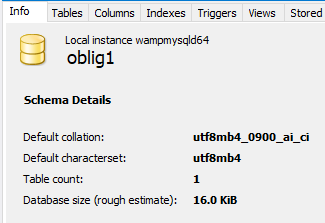
\includegraphics[scale=1]{op1a.png}
\end{figure}

\subsection*{b)}
For å lage tabellen "Film", så bruker jeg følgende sql:
\begin{sql}
oblig1> CREATE TABLE Oblig1.Film (
            FNr INTEGER UNSIGNED NOT NULL,
            Tittel VARCHAR(40) NOT NULL,
            År SMALLINT UNSIGNED,
            Land VARCHAR(40),
            Sjanger VARCHAR(20),
            Alder TINYINT UNSIGNED,
            Tid SMALLINT UNSIGNED,
            Pris DECIMAL(5, 2),
            PRIMARY KEY (FNr)
        )
[2022-09-11 17:25:37] completed in 19 ms
\end{sql}

\newpage
som resulterer i
\begin{figure}[H]
\centering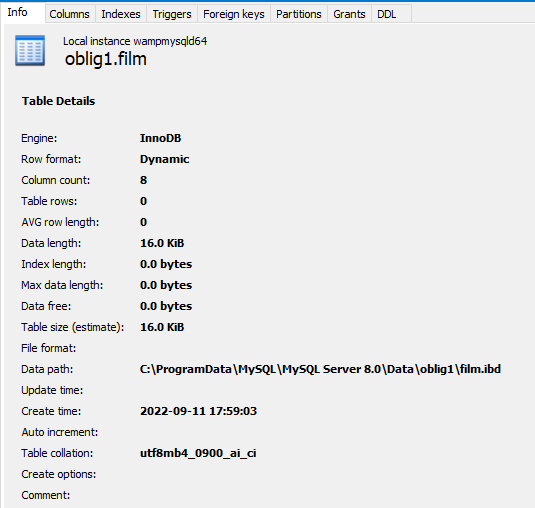
\includegraphics[scale=1]{op1b.png}
\end{figure}

\subsection*{c)}
Jeg legger til dataene fra tabellen i boken med følgende sql:
\begin{sql}
oblig1> INSERT INTO Oblig1.Film
        VALUES (1, 'Casablanca', 1942, 'USA', 'Drama', 15, 102, 149.00),
               (2, 'Fort Apachea', 1948, 'USA', 'Western', 15, 127, NULL),
               (3, 'Apocalypse Now', 1979, 'USA', 'Action', 18, 155, 123.00),
               (4, 'Streets of Fire', 1984, 'USA', 'Action', 15, 93, NULL),
               (5, 'High Noon', 1952, 'USA', 'Western', 15, 85, 123.00),
               (6, 'Cinema Paradiso', 1988, 'Italia', 'Komedie', 11, 123, NULL),
               (7, 'Asterix hos britene', 1988, 'Frankrike', 'Tegnefilm', 7, 78, 149.00),
               (8, 'Veiviseren', 1987, 'Norge', 'Action', 15, 96, 87.00),
               (9, 'Salmer fra kjøkkenet', 2002, 'Norge', 'Komedie', 7, 80, 149.00),
               (10, 'Anastasia', 1997, 'USA', 'Tegnefilm', 7, 94, 123.00),
               (11, 'La Grande bouffe', 1973, 'Frankrike', 'Drama', 15, 129, 87.00),
               (12, 'Blues Brothers 2000', 1998, 'USA', 'Komedie', 11, 124, 135.00),
               (13, 'Beatles: Help', 1965, 'Storbritannia', 'Musikk', 11, 144, NULL)
[2022-09-11 18:13:34] 13 rows affected in 6 ms
oblig1> SELECT * FROM Oblig1.Film
[2022-09-11 18:19:18] 13 rows retrieved starting from 1 in 39 ms (execution: 5 ms, fetching: 34 ms)
\end{sql}

\newpage
som resulterer i
\begin{figure}[H]
\centering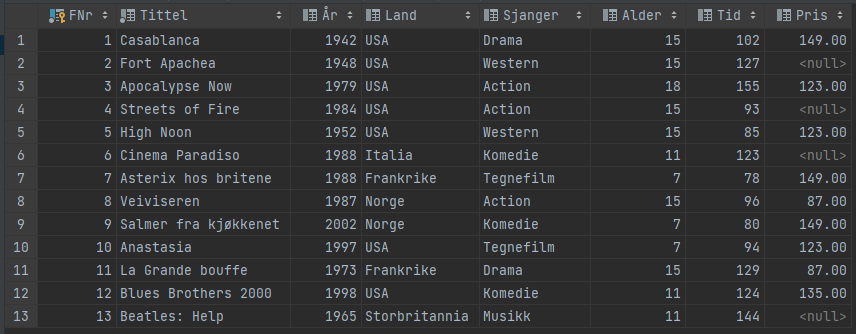
\includegraphics[width=\columnwidth]{op1c.png}
\end{figure}

\subsection*{d)}
For å finne tittel, sjanger og pris for filmer produsert i eller etter 1988, og sortere resultatet synkende etter pris, så bruker jeg følgende spørring:
\begin{sql}
oblig1> SELECT Tittel, Sjanger, Pris
        FROM Oblig1.Film
        WHERE År >= 1988
        ORDER BY Pris DESC
[2022-09-11 18:13:38] 5 rows retrieved starting from 1 in 44 ms (execution: 5 ms, fetching: 39 ms)
\end{sql}
som resulterer i
\begin{figure}[H]
\centering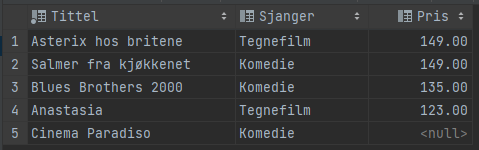
\includegraphics[scale=1]{op1d.png}
\end{figure}

\subsection*{e)}
For å hente alle kolonner for filmer som mangler pris, sortert først etter aldersgrense og så alfabetisk etter sjanger, så bruker jeg følgende spørring:
\begin{sql}
oblig1> SELECT * FROM Oblig1.Film
        WHERE Pris IS NULL
        ORDER BY Alder, Sjanger ASC
[2022-09-11 18:26:48] 4 rows retrieved starting from 1 in 52 ms (execution: 18 ms, fetching: 34 ms)
\end{sql}
\newpage
som resulterer i
\begin{figure}[H]
\centering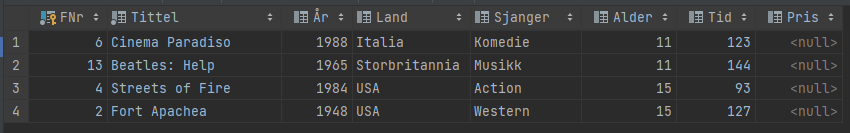
\includegraphics[width=\columnwidth]{op1e.png}
\end{figure}

\subsection*{f)}
Jeg finner antall filmer i hver sjanger som er til salgs, og totalpris per sjanger, ved hjelp av følgende spørring:
\begin{sql}
oblig1> SELECT Sjanger, COUNT(Sjanger) AS 'Antall filmer', SUM(Pris) AS 'Totalpris'
        FROM Oblig1.Film
        WHERE Pris IS NOT NULL
        GROUP BY Sjanger
        ORDER BY Sjanger ASC
[2022-09-11 18:51:56] 5 rows retrieved starting from 1 in 30 ms (execution: 5 ms, fetching: 25 ms)
\end{sql}
som resulterer i
\begin{figure}[H]
\centering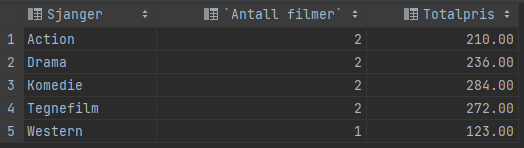
\includegraphics[width=\columnwidth]{op1f.png}
\end{figure}

\subsection*{g)}
Jeg legger til data for filmen "Ghost in the Shell (1995)" ved følgende spørring:
\begin{sql}
oblig1> INSERT INTO Oblig1.Film
        VALUE (14, 'Ghost in the Shell', 1995, 'Japan', 'Tegnefilm', 13, 83, 95.00)
[2022-09-11 19:02:07] 1 row affected in 19 ms
oblig1> SELECT * FROM Oblig1.Film
        WHERE Tittel = 'Ghost in the Shell'
[2022-09-11 19:04:31] 1 row retrieved starting from 1 in 29 ms (execution: 4 ms, fetching: 25 ms)
\end{sql}
som resulterer i
\begin{figure}[H]
\centering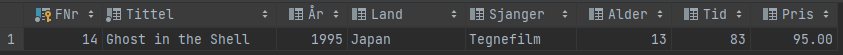
\includegraphics[width=\columnwidth]{op1g.png}
\end{figure}

\newpage
\subsection*{h)}
Bruker følgende sql for å korrigere tittelen film nummer \(5\) fra 'High Noon' til 'High Moon':
\begin{sql}
oblig1> UPDATE Oblig1.Film
        SET Tittel = 'High Moon'
        WHERE Tittel = 'High Noon'
[2022-09-11 19:15:28] 1 row affected in 7 ms
oblig1> SELECT FNr, Tittel
        FROM Oblig1.Film
        WHERE Tittel = 'High Moon'
[2022-09-11 19:16:32] 1 row retrieved starting from 1 in 30 ms (execution: 5 ms, fetching: 25 ms)
\end{sql}
som resulterer i
\begin{figure}[H]
\centering
\includegraphics[scale=1]{op1h.png}
\end{figure}

\subsection*{i)}
Øker prisen med \(10\%\) på action-filmer med følgende kode:
\begin{sql}
oblig1> UPDATE Oblig1.Film
        SET Pris = Pris * 1.1
        WHERE Sjanger = 'Action'
[2022-09-11 19:23:18] 3 rows affected in 6 ms
oblig1> SELECT Sjanger, Tittel, Pris
        FROM Oblig1.Film
        WHERE Sjanger = 'Action'
        ORDER BY Tittel ASC
[2022-09-11 19:27:54] 3 rows retrieved starting from 1 in 31 ms (execution: 4 ms, fetching: 27 ms)
\end{sql}
som resulterer i
\begin{figure}[H]
\centering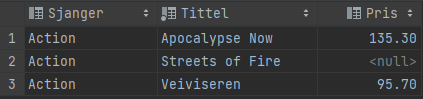
\includegraphics[scale=1]{op1i.png}
\end{figure}

\section*{j}
Sletter filmen 'Anastasia':
\begin{sql}
oblig1> DELETE
        FROM Oblig1.Film
        WHERE Tittel = 'Anastasia'
[2022-09-11 19:34:24] 1 row affected in 21 ms
oblig1> SELECT Tittel
        FROM Oblig1.Film
        ORDER BY Tittel ASC
[2022-09-11 19:35:25] 13 rows retrieved starting from 1 in 35 ms (execution: 17 ms, fetching: 18 ms)
\end{sql}
\newpage
som resulterer i
\begin{figure}[H]
\centering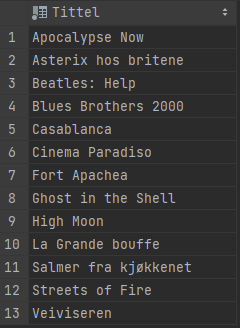
\includegraphics[scale=1]{op1j.png}
\end{figure}

\section*{Oppgave 2}
\subsection*{a)}
Lager tabellen 'Kunde':
\begin{sql}
oblig1> CREATE TABLE Oblig1.Kunde (
            KNr INTEGER UNSIGNED NOT NULL,
            Fornavn VARCHAR(50),
            Etternavn VARCHAR(50),
            Adresse VARCHAR(100),
            PostNr SMALLINT UNSIGNED,
            PRIMARY KEY (KNr)
        )
[2022-09-11 19:45:51] completed in 37 ms
oblig1> SELECT *
        FROM Oblig1.kunde
[2022-09-11 19:47:38] 0 rows retrieved in 29 ms (execution: 4 ms, fetching: 25 ms)
\end{sql}
som resulterer i
\begin{figure}[H]
\centering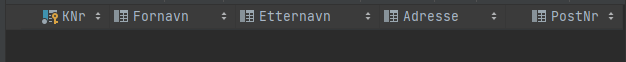
\includegraphics[scale=1]{op2a.png}
\end{figure}

\subsection*{b)}
Legger til data for tre kunder:
\begin{sql}
oblig1> INSERT INTO Oblig1.Kunde
        VALUES (10001, 'Kari', 'Mo', 'Moldegata 21 H0402', 0445),
               (10002, 'Geir', 'Gallestein', 'Grønnegata 68 H0304', 2317),
               (10003, 'Reidun', 'Roterud', 'Hylleråsvegen 11', 2440)
[2022-09-11 19:56:01] 3 rows affected in 6 ms
oblig1> SELECT *
        FROM Oblig1.Kunde
[2022-09-11 19:56:03] 3 rows retrieved starting from 1 in 35 ms (execution: 5 ms, fetching: 30 ms)
\end{sql}
som resulterer i
\begin{figure}[H]
\centering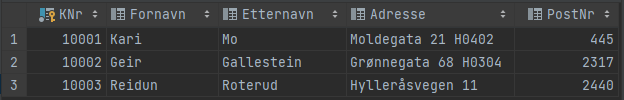
\includegraphics[width=\columnwidth]{op2b.png}
\end{figure}

\subsection*{c)}
Lager en faktura-tabell med kolonner for fakturanummer, kundenummer, beløp, opprettelsesdato, forfallsdato, filmnummer og betalt. Fakturanummeret er unikt til hver faktura, og brukes derfor som primærnøkkel. Kundenummeret er en fremmednøkkel knyttet til hovednøkkelen i kunde-tabellen, slik at man vet hvilken kunde som har utført bestillingen. Filmnummeret er også en fremmednøkkel knyttet til hovednøkkelen i film-tabellen, slik at man vet hvilken film som er blitt leid. Til slutt har vi en bool i betalt som er True, hvis fakturaen er betalt og false hvis den ikke er betalt.

Ingen av nøklene kan være NULL, siden fakturaen må ha et fakturanummer, må kunne knyttes til en leietager, og må kunne knyttes til produktet som ble utleid, ellers er det ikke en gyldig faktura. Jeg lar beløp være NULL ved default, da må prisen føres inn manuelt. Jeg valgte å ha prisen som DECIMAL(7, 2), siden da kan beløp pål opptil 99.999,- brukes. Datoene skal være på formatet 'YYYY-MM-DD', f.eks. '2022.04.11', og de kan ikke være NULL, for da kan ikke transaksjonen tidfestes, og er ugyldig. Hvis en faktura ikke opprettes med utfylte datoer, så blir opprettelsesdatoen lik datoen når fakturaen ble lagt til i tabellen, og forfallsdato blir 14 dager fra opprettelsesdato.

\begin{sql}
oblig1> CREATE TABLE Oblig1.Faktura
        (
            FakturaNr        INTEGER UNSIGNED NOT NULL,
            KundeNr          INTEGER UNSIGNED NOT NULL,
            FilmNr           INTEGER UNSIGNED NOT NULL,
            Beløp            DECIMAL(7, 2)             DEFAULT NULL,
            Opprettelsesdato DATE             NOT NULL DEFAULT (CURRENT_DATE),
            Forfallsdato     DATE             NOT NULL DEFAULT (Opprettelsesdato + INTERVAL 14 DAY),
            Betalt BOOL DEFAULT (FALSE),
            PRIMARY KEY (FakturaNr),
            FOREIGN KEY (KundeNr) REFERENCES Oblig1.Kunde (KNr),
            FOREIGN KEY (FilmNr) REFERENCES Oblig1.Film (FNr)
        )
[2022-09-11 22:04:56] completed in 24 ms
\end{sql}

\newpage
\subsection*{d)}
Jeg legger til to fakturaer for Kari Mo:
\begin{sql}
oblig1> INSERT INTO Oblig1.Faktura (FakturaNr, KundeNr, FilmNr, Beløp, Opprettelsesdato, Betalt)
            VALUES
                (
                 10001,
                 (SELECT KNr FROM Oblig1.Kunde WHERE Fornavn = 'Kari' AND Etternavn = 'Mo'),
                 14,
                 (SELECT Pris FROM Oblig1.Film WHERE FNr = 14),
                 '2021-12-30',
                 TRUE
                ),
                (
                 10002,
                 (SELECT KNr FROM Oblig1.Kunde WHERE Fornavn = 'Geir' AND Etternavn = 'Gallestein'),
                 11,
                 (SELECT Pris FROM Oblig1.Film WHERE FNr = 11),
                 '2022-04-01',
                 TRUE
                ),
                (
                 13592,
                 (SELECT KNr FROM Oblig1.Kunde WHERE Fornavn = 'Kari' AND Etternavn = 'Mo'),
                 5,
                 (SELECT Pris FROM Oblig1.Film WHERE FNr = 5),
                 CURRENT_DATE,
                 FALSE
                )
[2022-09-11 22:13:52] 3 rows affected in 7 ms
oblig1> SELECT *
        FROM Oblig1.Faktura
[2022-09-11 22:13:59] 3 rows retrieved starting from 1 in 26 ms (execution: 5 ms, fetching: 21 ms)
\end{sql}
som resulterer i
\begin{figure}[H]
\centering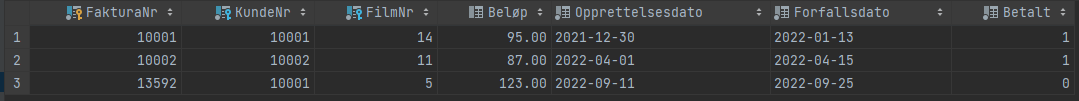
\includegraphics[width=\columnwidth]{op2d.png}
\end{figure}

\subsection*{e)}
Finner Kari Mo sine fakturaer ved navn:
\begin{sql}
oblig1> SELECT *
        FROM Oblig1.Faktura
        WHERE KundeNr = (SELECT KNr FROM Oblig1.Kunde WHERE Fornavn = 'Kari' AND Etternavn = 'Mo')
[2022-09-11 22:18:13] 2 rows retrieved starting from 1 in 38 ms (execution: 4 ms, fetching: 34 ms)
\end{sql}
som resulterer i
\begin{figure}[H]
\centering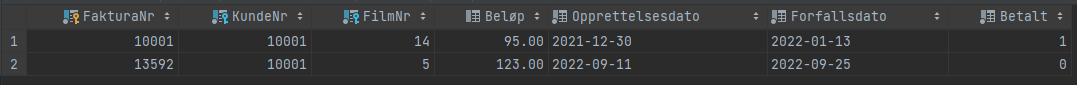
\includegraphics[width=\columnwidth]{op2e.png}
\end{figure}

\subsection*{f)}
Lagt til forretningsregel for beløpet, slik at beløpet må være i intervallet \(\left[0, 10.000\right]\):
\begin{sql}
oblig1> ALTER TABLE Oblig1.Faktura
            ADD CONSTRAINT Beløpsintervall
            CHECK ( Beløp >= 0.00 AND Beløp <= 10000.00)
[2022-09-11 22:28:29] 3 rows affected in 55 ms
\end{sql}

\subsection*{g)}
Prøver å legge inn faktura med ulovlig beløp:
\begin{sql}
oblig1> INSERT INTO Oblig1.Faktura (FakturaNr, KundeNr, FilmNr, Beløp)
        VALUE (1010, 10003, 1, 10000.69)
[2022-09-11 22:38:57] [HY000][3819] Check constraint 'Beløpsintervall' is violated.
[2022-09-11 22:38:57] [HY000][3819] Check constraint 'Beløpsintervall' is violated.
oblig1> SELECT *
        FROM Oblig1.Faktura
[2022-09-11 22:39:03] 3 rows retrieved starting from 1 in 53 ms (execution: 6 ms, fetching: 47 ms)
\end{sql}
Her fikk jeg en feilmelding om at forretningsregelen er brutt, og ved å printe tabellen så ser jeg at den ulovlige fakturaen ikke ble lagt til:
\begin{figure}[H]
\centering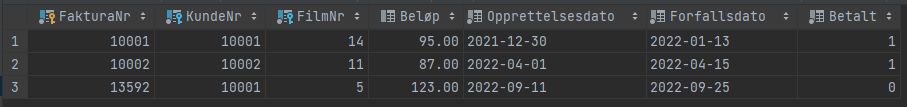
\includegraphics[width=\columnwidth]{op2f.png}
\end{figure}

\subsection*{h)}
Reduserer beløpet med en faktor \(10\), og kjører koden på nytt. Denne gang kommer ingen feilmelding:
\begin{sql}
oblig1> INSERT INTO Oblig1.Faktura (FakturaNr, KundeNr, FilmNr, Beløp)
        VALUE (1010, 10003, 1, 1000.69)
[2022-09-11 22:39:01] 1 row affected in 5 ms
oblig1> SELECT *
        FROM Oblig1.Faktura
[2022-09-11 22:39:04] 4 rows retrieved starting from 1 in 29 ms (execution: 3 ms, fetching: 26 ms)
\end{sql}
Jeg ser at den korrigerte fakturaen ble lagt til:
\begin{figure}[H]
\centering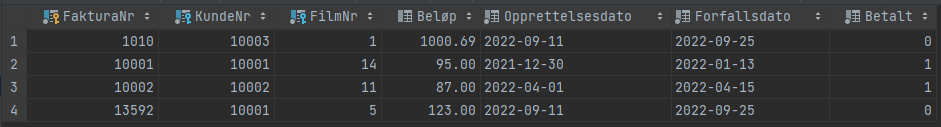
\includegraphics[width=\columnwidth]{op2h.png}
\end{figure}

\newpage
\section*{Oppgave 3}
\subsection*{a)}
Dokumentasjon av \verb+SUBSTRING_INDEX()+:
\begin{figure}[H]
\centering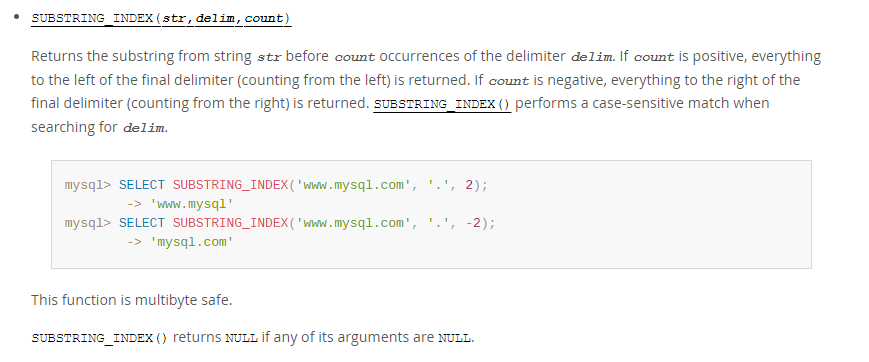
\includegraphics[width=\columnwidth]{op3a.png}
\end{figure}
Hentet fra:
ORACLE. (2022). MySQL 8.0 Reference Manual: 12.8 String Functions and Operators [Documentation]. MySQL. \url{https://dev.mysql.com/doc/refman/8.0/en/string-functions.html#function_substring-index}

\subsection*{b)}
For å vise at jeg kan bruke \verb+SUBSTRING_INDEX()+:, så bruker jeg den til å hente de to mitterste ordene i tittelen til film nummer \(14\) (Ghost in the Shell). Først lager jeg et uttrykk som deler tittelen ved mellomrom, og returnerer en streng med teksten opp til tredje mellomrom:
\begin{sql}
oblig1> SELECT SUBSTRING_INDEX((SELECT Tittel FROM Oblig1.Film WHERE FNr = 14), ' ', 3)
[2022-09-11 23:43:05] 1 row retrieved starting from 1 in 21 ms (execution: 5 ms, fetching: 16 ms)
\end{sql}
Den returnerer som forventet teksten 'Ghost in the':
\begin{figure}[H]
\centering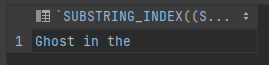
\includegraphics[scale=1]{op3b1.png}
\end{figure}

Jeg kan så bruke det tidligere nevnte sql-uttrykket som input-teksten til \verb+SUBSTRING_INDEX()+, og count lik \(-2\), slik at jeg henter tekst fra slutten av input-teksten til første mellomrom:
\begin{sql}
oblig1> SELECT SUBSTRING_INDEX((SELECT SUBSTRING_INDEX((SELECT Tittel FROM Oblig1.Film WHERE FNr = 14), ' ', 3)), ' ', -2)
[2022-09-11 23:43:05] 1 row retrieved starting from 1 in 44 ms (execution: 6 ms, fetching: 38 ms)
\end{sql}
Da for jeg som forventet teksten 'in the':
\begin{figure}[H]
\centering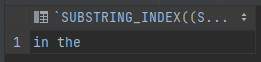
\includegraphics[scale=1]{op3b2.png}
\end{figure}

\section*{Oppgave 4}
\subsection*{a)}
Henter all data fra \verb+information_schema.TABLES+ med følgende spørring:
\begin{sql}
oblig1> SELECT *
        FROM information_schema.TABLES
[2022-09-11 23:55:12] 339 rows retrieved starting from 1 in 223 ms (execution: 52 ms, fetching: 171 ms)
\end{sql}
Jeg ser så at alle tre tabellene i Oblig1 databasen har en 'InnoDB' som verdi i ENGINE-kolonnen:
\begin{figure}[H]
\centering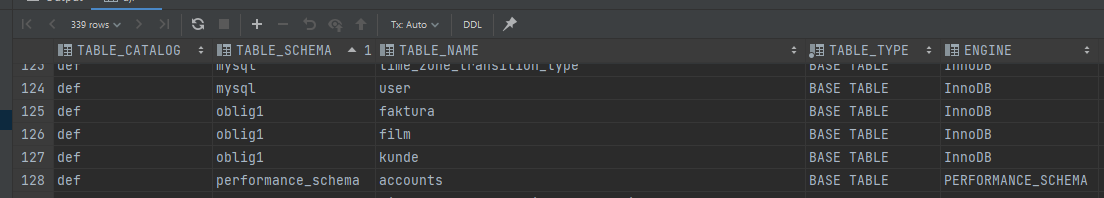
\includegraphics[width=\columnwidth]{op4a.png}
\end{figure}

\subsection*{b)}
Jeg fant dokumentasjonen for \verb+information_schema+ databasen her:
ORACLE. (2022). MySQL Information Schema [Documentation]. MySQL. \sloppy\url{https://dev.mysql.com/doc/mysql-infoschema-excerpt/8.0/en/}

\subsection*{c)}
Jeg sjekker tabellen for databasemotorer, for å se hvaslags informasjon er lagret om de:
\begin{sql}
oblig1> SELECT *
        FROM information_schema.ENGINES
[2022-09-12 00:12:55] 9 rows retrieved starting from 1 in 29 ms (execution: 5 ms, fetching: 24 ms)
\end{sql}
som gir:
\begin{figure}[H]
\centering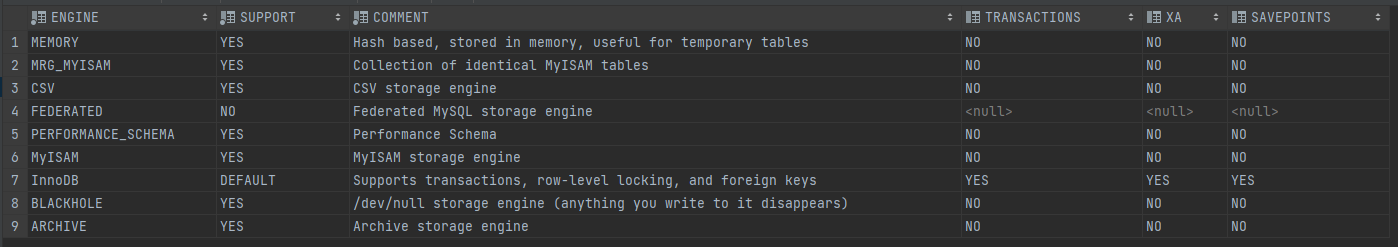
\includegraphics[width=\columnwidth]{op4c1.png}
\end{figure}

Jeg sjekker også tabellen for forretningsregler for å se hvordan den jeg lagde i oppgave 2. f) blir lagret:
\begin{sql}
oblig1> SELECT *
        FROM information_schema.CHECK_CONSTRAINTS
[2022-09-12 00:12:55] 1 row retrieved starting from 1 in 51 ms (execution: 4 ms, fetching: 47 ms)
\end{sql}
som gir:
\begin{figure}[H]
\centering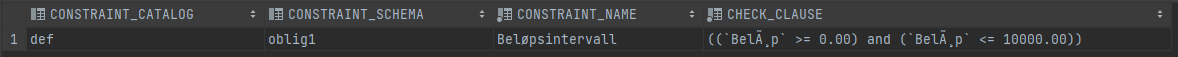
\includegraphics[width=\columnwidth]{op4c2.png}
\end{figure}
Interessant å se at den ikke lagrer 'ø' riktig i selve betingelsen, men uten at det skaper problemer for databasens operasjon.

\section*{Oppgave 5}
\subsection*{a)}
Etter å ha gjort denne obligen, så har ikke forståelsen min for konseptet bak relasjonsdatabaser endret seg særlig. Dette er fordi jeg allerede hadde lært meg mye av teorien tidligere. Derimot har min forståelse, samt beherskelse av SQL spesifikt blitt en god del bedre, og jeg har fått en god forståelse av hvordan databasene oppererer i MySQL implementasjonen.

\subsection*{b)}
Jeg ser nå hvordan jeg skal gå fram for å dele opp data i tabeller med relaterte felt, og hvordan jeg kan knytte disse tabellene sammen med bruk av fremmednøkler. Samt at jeg nå har erfaring med å designe en SQL-database, og derfor føler meg mer rustet til å designe fremtidige databaser.

\end{document}